\documentclass{article}

%=======================Title settings=======================
\title{SWT - Mandatory Assigment 3 : Integration Test}
\author{Gruppe 16}
\date{\today}

%=======================Use Package==========================
\usepackage[utf8]{inputenc}
\usepackage{natbib}
\usepackage{graphicx}
\usepackage{float}
\usepackage{amsmath}
\usepackage{amsfonts}
\usepackage{amssymb}
\usepackage{graphicx}
\usepackage{booktabs}
\usepackage{listings}
\usepackage{xcolor}
\usepackage{hyperref}
\usepackage{comment}
\usepackage{hyperref}
%=======================Package settings=======================

\hypersetup{
    colorlinks,
    citecolor=black,
    filecolor=black,
    linkcolor=black,
    urlcolor=blue
}

\lstset{
  language=Matlab,                % choose the language of the code
  numbers=left,                   % where to put the line-numbers
  stepnumber=1,                   % the step between two line-numbers.        
  numbersep=5pt,                  % how far the line-numbers are from the code
  backgroundcolor=\color{white},  % choose the background color. You must add \usepackage{color}
  showspaces=false,               % show spaces adding particular underscores
  showstringspaces=false,         % underline spaces within strings
  showtabs=false,                 % show tabs within strings adding particular underscores
  tabsize=2,                      % sets default tabsize to 2 spaces
  captionpos=b,                   % sets the caption-position to bottom
  %caption={Kode udsnit fra main.c programmet til opgave 1},
  %label=mainOpg1
  breaklines=true,                % sets automatic line breaking
  breakatwhitespace=true,         % sets if automatic breaks should only happen at whitespace
  belowcaptionskip=1\baselineskip,
  %frame=L,
  xleftmargin=\parindent,
  basicstyle=\footnotesize\ttfamily,
  keywordstyle=\bfseries\color{blue},
  commentstyle=\itshape\color{teal},
  identifierstyle=\color{black},
  stringstyle=\color{red},
}


%=======================Page settings=======================
\topmargin 0.0cm
\oddsidemargin 0.2cm
\textwidth 16cm 
\textheight 21cm
\footskip 1.0cm


\begin{document}
%=======================Title========================
\maketitle

\begin{table}[H]
\centering
\begin{tabular}{|l|l|l|}
\hline
\textbf{Navn}       & \textbf{Studieretning} & \textbf{Student Number} \\ \hline
Sivert Sømmer Sagmo & IKT                    & 201608544             \\ \hline
Glenn Laursen & IKT                    & 201703930             \\ \hline
Saeed Soltani & IKT                    & 201710716             \\ \hline
\end{tabular}
\end{table}

Github Repository : \url{https://github.com/glennlaursen/SWT_Assignment3_GR16/}

Jenkins Unit Test : \url{http://ci3.ase.au.dk:8080/job/SWT_E2019_16_MicroWave/}

Jenkins Integration Test : \url{http://ci3.ase.au.dk:8080/job/SWT_E2019_16_MicroWave_Integration/}

\tableofcontents
\pagebreak
%=======================Sections=======================

\section{Dependency Tree}
\begin{figure}[H]
	\centering
	\includegraphics[width=1\linewidth]{"../Diagrams/DependencyTree_Microwave - Updatet - Numbered"}
	\caption{Dependency Tree for Microwave program, with step numbers}
	\label{fig:dependencytreemicrowave}
\end{figure}
\section{Dependency Plan}

\begin{figure}[H]
	\centering
	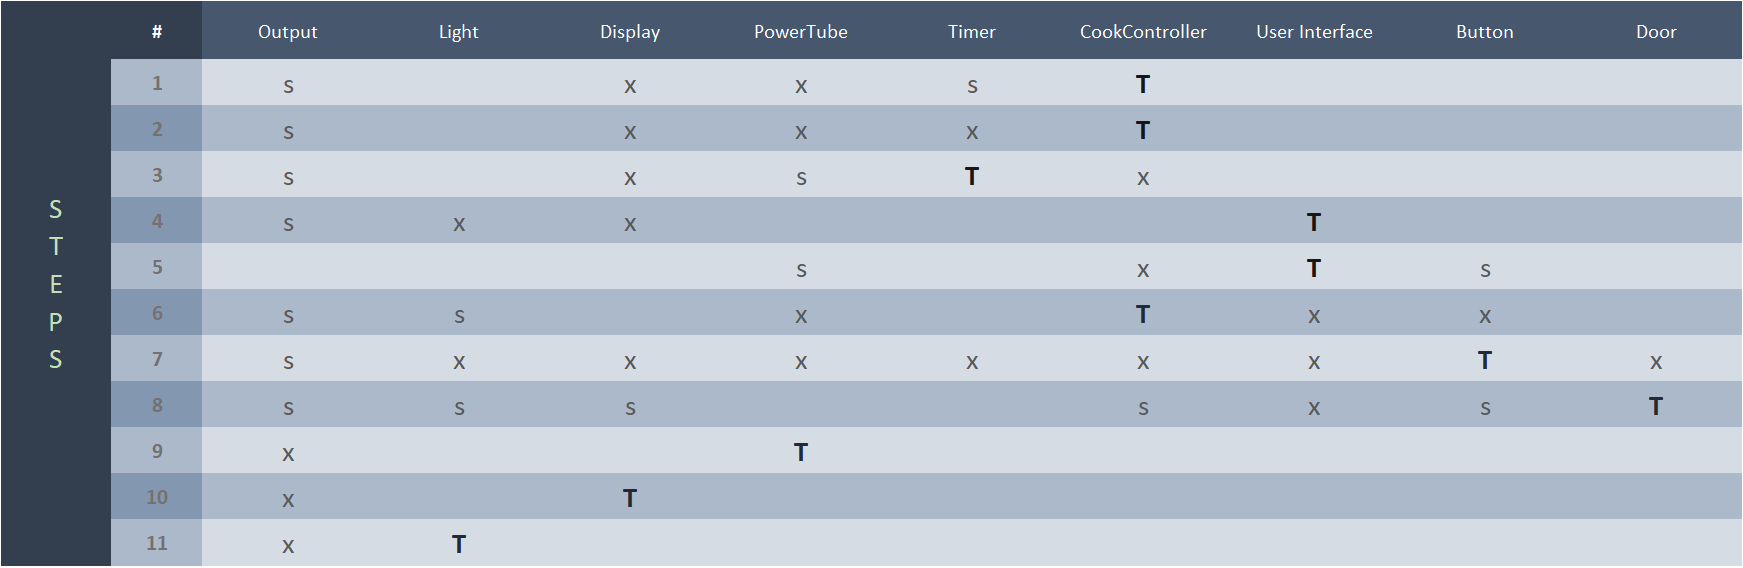
\includegraphics[width=1\linewidth]{../Diagrams/IntegrationPlan}
	\caption[Integration Plan]{Integrationsplan. Nummerne tilsvarer de i figure \ref{fig:dependencytreemicrowave}. T er unit under test, s er moduler der er fakes og x er moduler der er inkluderet i testen.}
	\label{fig:integrationplan}
\end{figure}

\subsection{Valg for Integrations plan}
%begrundelse hvorfor bedste patterns (første udkast bottom up, top-down)
hovedpointen i bottom up metoden er at man kan integrations teste systemet ved start af de komponenter med færrest afhængigheder. dvs komponenter med færrest afhængigheder testes først. Når disse komponenter er blevet testet og godkendt så kan man rykker videre til de næste komponenter indtil hele systemet er blevet testet. \medskip
Fordelen ved bottom op er at vi kan hurtigt går i gang med at integerer en smule af systemet. der kan integeres parallelt hvis projektet er stort. I andre ord, så kan der være flere udvikler der arbejder samtidigt på systemets test. Da de ikke er afhængig af de andre udviklers integrationstest. \medskip
Set ud fra vores afhængighedstræ er der en del komponenter der afhænger af andre komponenter i afhængigheds træet. derfor tænker vi at det vil være oplagt at anvende bottom op metoden.


\section{Fejl rettelser}

\subsection{Powertube}
i funktionen TurnOn i klassen PowerTube var fejlen at i stedet for enheden var i Watt så var enheden i procent. Valideringen i if sætningen blev ændret fra 50 til 700. hvor der originalt stod 1 til 100. OutputLine der skal procent ændres til Watt
\subsection{Timer}
i klassen Timer og UserInterface der er enhederne ikke konsekvent. hele tiden så vi har ændret i Timer klassen i funktionen OnTimerEvent hvor TimeRemaining er ændret til 1 hvor den var 1000 før 
\subsection{Unit Test PowerTube og Timer}
vi har rettet de fejl der hører til under de fejl vi fandt i de tilhørende boundary klasser. f.eks. i Unit testen TurnOn\_HighPower\_ThrowsExpection ændrede vi power fra 101 til 701.

\subsection{Diagrammer}
fra Set time til Cooking i state diagrammet så er der ikke staten Turn On light når man cooker. Men det er der i sekvens diagrammet.

%=======================Ex. Inserts====================

%\begin{figure}[h!]
%\centering
%\includegraphics[scale=1.7]{universe}
%\caption{The Universe}
%\label{fig:universe}
%\end{figure}

%\begin{lstlisting}[caption=Caption here]
%\end[lstlisting]

% \begin{equation}
%     H(s) = \frac{s + \omega_1}{s + \omega_2}
%     \label{eq:3.14}
% \end{equation}



%\bibliographystyle{plain}
%\bibliography{references}
\end{document}